%%%%%%%%%%%%%%%%%%%%%%%%%%%%%%%%%%%%%%%%%%%%%%%%%%%%%%%%%%%%%%%%%%%%%%%%%%%%%%%%%%%%%%%%
%% tikz draw a 3D representation of matrices for "image"
%% the tikz code 
%%%%%%%%%%%%%%%%%%%%%%%%%%%%%%%%%%%%%%%%%%%%%%%%%%%%%%%%%%%%%%%%%%%%%%%%%%%%%%%%%%%%%%%%
\newcommand{\tikzcube}[5]{% width, height, depth, color, scale 
    \foreach \x in {0,...,#1}
    {   \draw (\x*#5 ,0  ,#5*#3 ) -- (\x*#5 ,#5*#2 ,#5*#3 );
      \draw (\x*#5 ,#5*#2 ,#5*#3 ) -- (\x*#5 ,#5*#2 ,0  );
    }
    \foreach \x in {0,#2}
     {   \draw (#5*#1 ,\x*#5 ,#5*#3 ) -- (#5*#1 ,\x*#5 ,0  );
       \draw (0  ,\x*#5 ,#5*#3 ) -- (#5*#1 ,\x*#5 ,#5*#3 );
     }
     \foreach \x in {0,#3}
     {   \draw (#5*#1 ,0  ,\x*#5 ) -- (#5*#1 ,#5*#2 ,\x*#5 );
       \draw (0  ,#5*#2 ,\x*#5 ) -- (#5*#1 ,#5*#2 ,\x*#5 );
     }
    \draw[fill=#4!50,opacity=0.5] (0,0,#5*#3) rectangle (#5*#1,#5*#2,#5*#3);
    \draw[fill=#4!50] (#5*#1,0,0) -- (#5*#1,#5*#2,0) -- (#5*#1,#5*#2,#5*#3) -- (#5*#1,0,#5*#3) -- cycle ;
}

%%%%%%%%%%%%%%%%%%%%%%%%%%%%%%%%%%%%%%%%%%%%%%%%%%%%%%%%%%%%%%%%%%%%%%%%%%%%%%%%%%%%%%%%
%% The wrapper in a tikzpicture : scale can be 0.25 
%%%%%%%%%%%%%%%%%%%%%%%%%%%%%%%%%%%%%%%%%%%%%%%%%%%%%%%%%%%%%%%%%%%%%%%%%%%%%%%%%%%%%%%% 
\newcommand{\tikzcuboid}[5]{% width, height, depth, color, scale 
  \begin{tikzpicture}
    \tikzcube{#1}{#2}{#3}{#4}{#5}
  \end{tikzpicture}
}
%%%%%%%%%%%%%%%%%%%%%%%%%%%%%%%%%%%%%%%%%%%%%%%%%%%%%%%%%%%%%%%%%%%%%%%%%%%%%%%%%%%%%%%%
%% Shifted
%%%%%%%%%%%%%%%%%%%%%%%%%%%%%%%%%%%%%%%%%%%%%%%%%%%%%%%%%%%%%%%%%%%%%%%%%%%%%%%%%%%%%%%% 
\newcommand{\shiftedtikzcube}[7]{% width, height, depth, color, scale, xshift, yshift
    \foreach \x in {0,...,#1}
    {   \draw (\x*#5 +#6,0+#7  ,#5*#3 ) -- (\x*#5 +#6 ,#5*#2+#7 ,#5*#3 );
      \draw (\x*#5 +#6 ,#5*#2+#7 ,#5*#3 ) -- (\x*#5 +#6 ,#5*#2+#7 ,0  );
    }
    \foreach \x in {0,#2}
     {   \draw (#5*#1 +#6 ,\x*#5+#7 ,#5*#3 ) -- (#5*#1 +#6 ,\x*#5+#7 ,0  );
       \draw (0 +#6  ,\x*#5 +#7,#5*#3 ) -- (#5*#1 +#6 ,\x*#5+#7 ,#5*#3 );
     }
     \foreach \x in {0,#3}
     {   \draw (#5*#1+#6,0 +#7 ,\x*#5 ) -- (#5*#1 +#6 ,#5*#2 +#7,\x*#5 );
       \draw (0 +#6,#5*#2+#7 ,\x*#5 ) -- (#5*#1 +#6,#5*#2+#7 ,\x*#5 );
     }
    \draw[fill=#4!50,opacity=0.5] (0 +#6,0+#7,#5*#3) rectangle (#5*#1 +#6,#5*#2+#7,#5*#3);
    \draw[fill=#4!50] (#5*#1 +#6,0+#7,0) -- (#5*#1 +#6,#5*#2+#7,0) -- (#5*#1 +#6,#5*#2+#7,#5*#3) -- (#5*#1 +#6,0+#7,#5*#3) -- cycle ;
}



\begin{frame}{Image classification}
  \begin{center}
    An image = (2D array of values) $\times$ (number of channels)
  \end{center}
  \begin{block}{2D array}
    The spatial structure:
    \begin{itemize}
    \item A 2D real space
    \item With distance 
    \end{itemize}
  \end{block}
  \begin{block}{Channels}
    \begin{itemize}
    \item For image : R,G,B
    \item In fluid mechanics: pression, velocity, ... 
    \item In general: different measures on the same spatial domain
    \end{itemize}
  \end{block}
  \begin{block}{Sources}
    Many figures and examples are inspired by, or extracted from the
    course of the Stanford course of Fei-Fei Li.
    \begin{flushright}
      \small \url{http://cs231n.stanford.edu/}
    \end{flushright}
  \end{block}
\end{frame}

\begin{frame}{Image classification}
  \begin{center}
    \tikz[baseline=0]{ \node at (-2,0)
      {\includegraphics[height=0.25\textheight]{figs/mnist_5.pdf}}; %
      \node at (-0.4,0) {$\rightarrow$}; \xvector{0}{-0.75}{6} }
    $\x \in \real^{784} \ \longrightarrow \class  \in\{0, 1,2, \ldots ,9
    \}$
  \end{center}
  Another example with a color image (3 channels) of $32\times32$ pixels
  \begin{center}
    \tikz[baseline=0]{
      \shiftedtikzcube{3}{10}{10}{green}{0.25}{0}{-1}; 
      \node at (1,0) {$\rightarrow$}; \xvector{2}{-1.25}{10} }
    $\x \in \real^{3072} \ \longrightarrow \class  \in\{0, 1,2, \ldots ,9
    \}$
  \end{center}
\end{frame}


\begin{frame}{A simple 2D-convolution}
  \framesubtitle{One input channel and one output channel}
  \begin{itemize}
  \item Image of $(7,7)$
  \item Kernel size of $(3,3)$
  \item Stride of $(2,2)$ along line and column
\end{itemize}
  \begin{columns}
    \column{0.7\textwidth}
    \begin{center}
      \only<1>{Filter applied at $l=1$ and $c=1$\\[1ex]}
      \only<2>{Filter applied at $l=1$ and $c=3$\\[1ex]}
      \only<3>{Filter applied at $l=1$ and $c=5$\\[1ex]}
      \only<4>{Filter applied at $l=3$ and $c=1$\\[1ex]}
      \begin{tikzpicture}[scale=0.5,every node/.style={scale=0.75}]
        % the window
        % offset for x and y of .5 + a bit more/less 
        \only<1>{
          \draw[fill=green!20,rounded corners] (0.45,-0.45) rectangle (3.55,-3.55); % green
        }
        \only<2>{
          \draw[fill=green!20,rounded corners] (2.45,-0.45) rectangle (5.55,-3.55); % green
        }
        \only<3>{
          \draw[fill=green!20,rounded corners] (4.45,-0.45) rectangle (7.55,-3.55); % green
        }
        \only<4>{
          \draw[fill=green!20,rounded corners] (0.45,-2.45) rectangle (3.55,-5.55); % green
        }
        %% the grid 
        \foreach \l in {1,2,...,7}%{8,7,...,1}
        \foreach \c in {1,2,...,7}
        {
          \draw (\c,-\l) +(-.5,-.5) rectangle ++(.5,.5);
          \draw (\c,-\l) node{$x_{\l,\c}$};
        }
      \end{tikzpicture}
    \end{center}

    \column{0.3\textwidth}
    \begin{center}
      The filter or kernel is $3\times 3 $\\[1ex]
      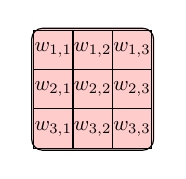
\begin{tikzpicture}[scale=0.5,every node/.style={scale=0.75}]
        % the window
        % offset for x and y of .5 + a bit more 
        \draw[fill=red!20,rounded corners] (0.45,-0.45) rectangle (3.55,-3.55); % green 
        
        %% the grid 
        \foreach \l in {1,2,3}
        \foreach \c in {1,2,3}
        {
          \draw (\c,-\l) +(-.5,-.5) rectangle ++(.5,.5);
          \draw (\c,-\l) node{$w_{\l,\c}$};
        }
      \end{tikzpicture}
    \end{center}
  \end{columns}
    $$
    \textrm{At position }l, \textrm{ and } c,\ {\color{red!70!black} h_{l,c}} = \sum_{i,j} {\color{red!70!black}w_{i,j}}\times  {\color{green!70!black}x_{l+i-1,c+j-1}}
  $$
\end{frame}

\begin{frame}{Convolution in 2D}
  \framesubtitle{The basics}
  \begin{columns}
    \column{0.6\textwidth}
    \begin{tabular}{lll}
      \begin{tabular}{c}
        \tikzcuboid{3}{10}{10}{green}{0.25}
      \end{tabular}
      & \begin{tabular}{c}
          $\longrightarrow$
        \end{tabular}
      & \begin{tabular}{c}
          \tikzcuboid{3}{3}{3}{red}{0.25}
        \end{tabular}
      \\
      $3\times 32\times 32$ image & &$3\times 5\times 5$ filter
    \end{tabular}
    \column{0.4\textwidth}
    Convolution of the filter  with the image:
    \begin{itemize}
    \item Sliding the filter along the two axis
    \item Computing the ``dot product'' at each step
    \item[$\rightarrow$] preserve the spatial structure along the channels
    \item[$\rightarrow$] each step extract a ``local'' and spatial feature
    \end{itemize}
  \end{columns}
\end{frame}

\begin{frame}{Convolution in 2D}
  \framesubtitle{With a single output channel}
  % \begin{center}
  %   \tikz[baseline=0]{
  %   \shiftedtikzcube{3}{10}{10}{green}{0.25}{0}{-1}; %% 
  %   \node at (1.5,0) {$\longrightarrow$}; 
  %   \shiftedtikzcube{3}{3}{3}{red}{0.25}{3}{0}; %%
  %   \node at (4.5,0) {$\longrightarrow$};
  %   \shiftedtikzcube{1}{8}{8}{red}{0.25}{6}{0}; %%
  % }
  % \end{center}


  \begin{center}
    \begin{tabular}{ccccc}
      \begin{tabular}{c}
        \tikzcuboid{3}{10}{10}{green}{0.25}
      \end{tabular}
      & \begin{tabular}{c}
          $\longrightarrow$
        \end{tabular}
      & \begin{tabular}{c}
          \tikzcuboid{3}{3}{3}{red}{0.25}
        \end{tabular}
      & \begin{tabular}{c}
          $\longrightarrow$
        \end{tabular}
      & \begin{tabular}{c}
          \tikzcuboid{1}{8}{8}{red}{0.25}
        \end{tabular}
      \\
      $3\times 32\times 32$ image & &$3\times 5\times 5$ filter & &$1 \times 28\times 28$ output 
    \end{tabular}
  \end{center}
\end{frame}

\begin{frame}{Convolution in 2D}
  \framesubtitle{Add a second output channel}
  % \begin{center}
  %   \tikz[baseline=0]{
  %   \shiftedtikzcube{3}{10}{10}{green}{0.25}{0}{-1}; %% 
  %   \node at (1.5,0) {$\longrightarrow$}; 
  %   \shiftedtikzcube{3}{3}{3}{red}{0.25}{3}{0}; %%
  %   \node at (4.5,0) {$\longrightarrow$};
  %   \shiftedtikzcube{1}{8}{8}{red}{0.25}{6}{0}; %%
  % }
  % \end{center}


  \begin{center}
    \begin{tabular}{ccccc}
      \begin{tabular}{c}
        \tikzcuboid{3}{10}{10}{green}{0.25}
      \end{tabular}
      & \begin{tabular}{c}
          $\longrightarrow$
        \end{tabular}
      & \begin{tabular}{c}
          \tikzcuboid{3}{3}{3}{red}{0.25}\\
          \tikzcuboid{3}{3}{3}{red}{0.25}\\
        \end{tabular}
      & \begin{tabular}{c}
          $\longrightarrow$
        \end{tabular}
      & \begin{tabular}{c}
          \tikzcuboid{2}{8}{8}{red}{0.25}
        \end{tabular}
      \\
      \begin{tabular}{c}
      $3\times 32\times 32$ \\image
      \end{tabular}
      &
      &\begin{tabular}{c}
         $2\times (3\times 5\times 5)$\\filters
       \end{tabular}
      &
      & \begin{tabular}{c}
          $2 \times 28\times 28$ \\ output
        \end{tabular}
    \end{tabular}
  \end{center}
\end{frame}


\begin{frame}{Motivation for convolution}
  \framesubtitle{Extract ``low level'' features}
  \begin{center}
    \only<1>{\includegraphics[width=0.8\textwidth]{../figs/image_and_filters_4}}
    \only<2>{\includegraphics[width=0.8\textwidth]{../figs/image_and_filters_1}}
    \only<3>{\includegraphics[width=0.8\textwidth]{../figs/image_and_filters_9}}
  \end{center}
\end{frame}


\begin{frame}{Max-pooling or Downsampling in 2D}
  \begin{block}{The goal}
    \begin{itemize}
    \item Convolution extracts local features (followed by non-linearity)
    \item Max-pooling acts as a selection, compression, or contraction operator
    \item The back-propagation promote feature saliency for each channel
    \end{itemize}
  \end{block}
  \begin{center}
    \includegraphics[width=0.7\textwidth]{../figs/pooling2D}
  \end{center}
\end{frame}

\begin{frame}{Architecture of deep convolution NNet for image processing}
  \framesubtitle{VGGNet~\cite{Simonyan15VGG}}
  \begin{center}
    \includegraphics[width=0.7\textwidth]{../figs/vgg16}
  \end{center}
  Conv. layers with kernel size of $3\times 3$, stride and padding,
  followed by pooling layers (max on $2\times 2$ with stride 2).
\end{frame}

\begin{frame}{Architecture of deep convolution NNet for image processing}
  \framesubtitle{A summary}
  \begin{block}{The basic block}
    \begin{itemize}
    \item A convolution layer with a ReLU activation followed by a max-pooling layer
    \item An alternative is two convolution layers in a Residual block (ResNet~\cite{He16Residual})
    \end{itemize}
  \end{block}
  \begin{center}
    \includegraphics[width=0.5\textwidth]{../figs/perf_imagenet.pdf}
  \end{center}
\end{frame}



\begin{frame}{Residual block }
  \begin{block}{Residual block}
    \begin{columns}
    \column{0.5\textwidth}
    From~\cite{He16Residual}
    \begin{itemize}
    \item Add a skip connection
    \item The model learn the "residual"
      $$
      \y = \mathcal{F}(\x) = \x + \mathcal{R}(\x)
      $$
    \end{itemize}
      \column{0.5\textwidth}
      \begin{center}
        \includegraphics[width=0.8\textwidth]{../figs/residual}
      \end{center}
    \end{columns}
    A simple version of highway networks~\cite{Srivastava15Highway}
  \end{block}
  \begin{block}{ResNet}
      \begin{center}
        \includegraphics[width=\textwidth]{../figs/resnet}
      \end{center}    
  \end{block}
\end{frame}


\begin{frame}{Residual block}
  \begin{block}{Forward}
    \begin{align*}
      \y &= \mathcal{F}(\x) = \x + \mathcal{R}(\x), \textrm{ or }\\
      \y &= \W_{s} \x + \mathcal{R}(\x), \textrm{ to adapt the dimension}
    \end{align*}
  \end{block}
  \begin{block}{Backward}
    Assume a residual block for the layer $l$ in the network. Training requires:
    \begin{itemize}
    \item $\frac{\partial l }{\partial\W\lid{l}}$ for the update of the layer
    \item $\frac{\partial l }{\partial\x\lid{l}}$ for the backpropagation
    \end{itemize}
    \begin{align*}
      \frac{\partial l }{\partial\x\lid{l}} &=       \frac{\partial l }{\partial\y\lid{l}} \times  \frac{\partial\y\lid{l}}{\partial\x\lid{l}}\\
                                            &= \frac{\partial l }{\partial\y\lid{l}} \times  (1+\frac{\partial\mathcal{R}(\x\lid{l})}{\partial\x\lid{l}})
    \end{align*}
  \end{block}
\end{frame}
